% Options for packages loaded elsewhere
\PassOptionsToPackage{unicode}{hyperref}
\PassOptionsToPackage{hyphens}{url}
%
\documentclass[
]{article}
\usepackage{lmodern}
\usepackage{amssymb,amsmath}
\usepackage{ifxetex,ifluatex}
\ifnum 0\ifxetex 1\fi\ifluatex 1\fi=0 % if pdftex
  \usepackage[T1]{fontenc}
  \usepackage[utf8]{inputenc}
  \usepackage{textcomp} % provide euro and other symbols
\else % if luatex or xetex
  \usepackage{unicode-math}
  \defaultfontfeatures{Scale=MatchLowercase}
  \defaultfontfeatures[\rmfamily]{Ligatures=TeX,Scale=1}
\fi
% Use upquote if available, for straight quotes in verbatim environments
\IfFileExists{upquote.sty}{\usepackage{upquote}}{}
\IfFileExists{microtype.sty}{% use microtype if available
  \usepackage[]{microtype}
  \UseMicrotypeSet[protrusion]{basicmath} % disable protrusion for tt fonts
}{}
\makeatletter
\@ifundefined{KOMAClassName}{% if non-KOMA class
  \IfFileExists{parskip.sty}{%
    \usepackage{parskip}
  }{% else
    \setlength{\parindent}{0pt}
    \setlength{\parskip}{6pt plus 2pt minus 1pt}}
}{% if KOMA class
  \KOMAoptions{parskip=half}}
\makeatother
\usepackage{xcolor}
\IfFileExists{xurl.sty}{\usepackage{xurl}}{} % add URL line breaks if available
\IfFileExists{bookmark.sty}{\usepackage{bookmark}}{\usepackage{hyperref}}
\hypersetup{
  pdftitle={Blossom Watch 2021},
  pdfauthor={Alan Millington},
  hidelinks,
  pdfcreator={LaTeX via pandoc}}
\urlstyle{same} % disable monospaced font for URLs
\usepackage[margin=1in]{geometry}
\usepackage{longtable,booktabs}
% Correct order of tables after \paragraph or \subparagraph
\usepackage{etoolbox}
\makeatletter
\patchcmd\longtable{\par}{\if@noskipsec\mbox{}\fi\par}{}{}
\makeatother
% Allow footnotes in longtable head/foot
\IfFileExists{footnotehyper.sty}{\usepackage{footnotehyper}}{\usepackage{footnote}}
\makesavenoteenv{longtable}
\usepackage{graphicx,grffile}
\makeatletter
\def\maxwidth{\ifdim\Gin@nat@width>\linewidth\linewidth\else\Gin@nat@width\fi}
\def\maxheight{\ifdim\Gin@nat@height>\textheight\textheight\else\Gin@nat@height\fi}
\makeatother
% Scale images if necessary, so that they will not overflow the page
% margins by default, and it is still possible to overwrite the defaults
% using explicit options in \includegraphics[width, height, ...]{}
\setkeys{Gin}{width=\maxwidth,height=\maxheight,keepaspectratio}
% Set default figure placement to htbp
\makeatletter
\def\fps@figure{htbp}
\makeatother
\setlength{\emergencystretch}{3em} % prevent overfull lines
\providecommand{\tightlist}{%
  \setlength{\itemsep}{0pt}\setlength{\parskip}{0pt}}
\setcounter{secnumdepth}{-\maxdimen} % remove section numbering

\title{Blossom Watch 2021}
\author{Alan Millington}
\date{2021-03-24 12:07:35}

\begin{document}
\maketitle

This table shows the total count of hashtags used where the various
combinations are used by twitter users. When the tweet does not contain
a hashtag, but contains the keywords it falls into the `no hashtag'
group. If any new hashtags are required to be tracked, please let me
know and this can be easily updated.

\begin{longtable}[]{@{}lr@{}}
\toprule
\begin{minipage}[b]{0.41\columnwidth}\raggedright
hashtag\strut
\end{minipage} & \begin{minipage}[b]{0.10\columnwidth}\raggedleft
count\strut
\end{minipage}\tabularnewline
\midrule
\endhead
\begin{minipage}[t]{0.41\columnwidth}\raggedright
blossom\strut
\end{minipage} & \begin{minipage}[t]{0.10\columnwidth}\raggedleft
2550\strut
\end{minipage}\tabularnewline
\begin{minipage}[t]{0.41\columnwidth}\raggedright
blossomwatch\strut
\end{minipage} & \begin{minipage}[t]{0.10\columnwidth}\raggedleft
1634\strut
\end{minipage}\tabularnewline
\begin{minipage}[t]{0.41\columnwidth}\raggedright
NationalTrust + BlossomWatch\strut
\end{minipage} & \begin{minipage}[t]{0.10\columnwidth}\raggedleft
36\strut
\end{minipage}\tabularnewline
\begin{minipage}[t]{0.41\columnwidth}\raggedright
EveryoneNeedsNature\strut
\end{minipage} & \begin{minipage}[t]{0.10\columnwidth}\raggedleft
314\strut
\end{minipage}\tabularnewline
\begin{minipage}[t]{0.41\columnwidth}\raggedright
No Hashtag (Text contains keywords)\strut
\end{minipage} & \begin{minipage}[t]{0.10\columnwidth}\raggedleft
1828\strut
\end{minipage}\tabularnewline
\bottomrule
\end{longtable}

\hypertarget{timeline}{%
\section{Timeline}\label{timeline}}

\hypertarget{tweets-by-day}{%
\subsection{Tweets by day}\label{tweets-by-day}}

Frequency of tweets broken down by day.
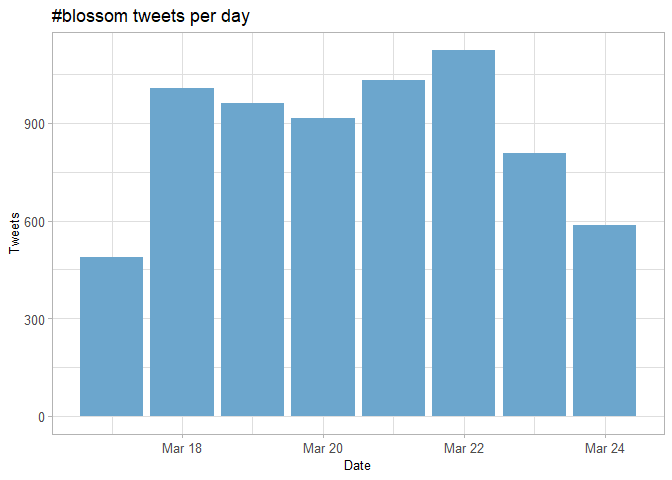
\includegraphics{twitter-blossom-watch-2021_files/figure-latex/tweets-by-day-1.pdf}

\hypertarget{tweets-by-day-and-time}{%
\subsection{Tweets by day and time}\label{tweets-by-day-and-time}}

Filtered for dates March, London time. Tweet frequency broken down by
day and hour of day.
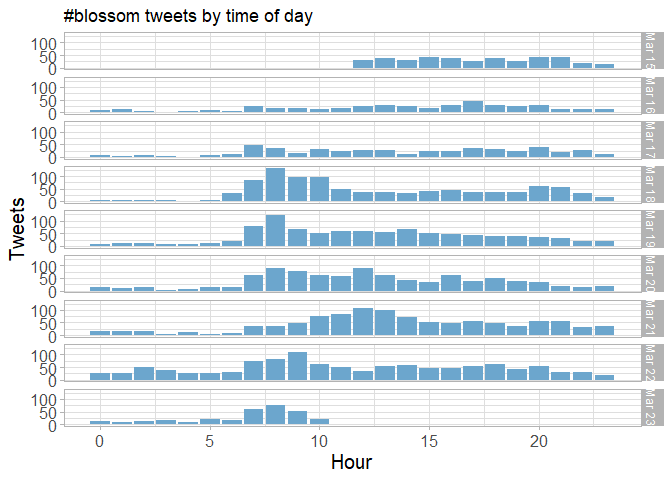
\includegraphics{twitter-blossom-watch-2021_files/figure-latex/tweets-by-day-hour-1.pdf}

\hypertarget{users}{%
\section{Users}\label{users}}

\hypertarget{top-tweeters}{%
\subsection{Top tweeters}\label{top-tweeters}}

Top twitter users that have tweeted more than 10 tweets containing the
\#blossom hashtag.
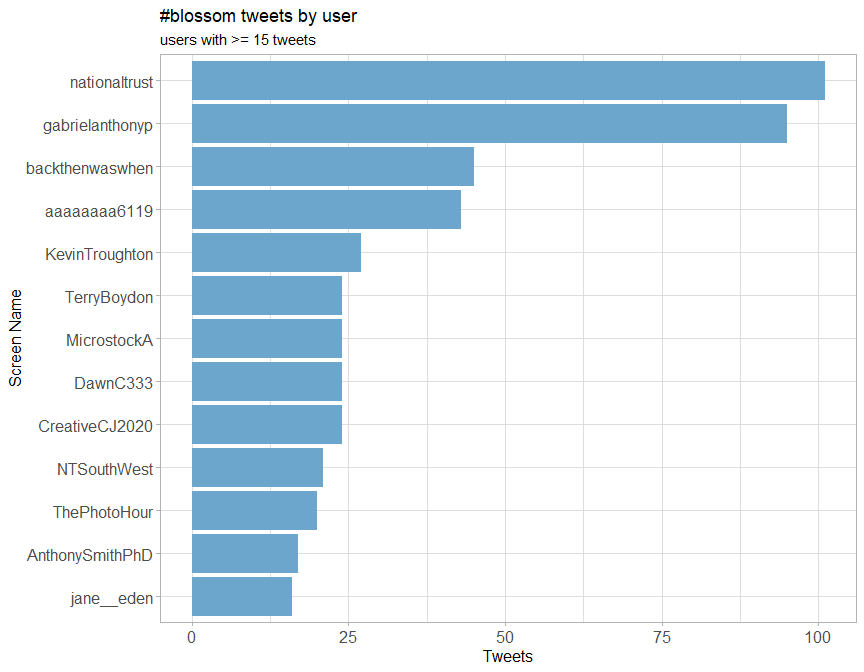
\includegraphics{twitter-blossom-watch-2021_files/figure-latex/tweets-top-users-1.pdf}

\hypertarget{sources}{%
\subsection{Sources}\label{sources}}

Breakdown of twitter source clients that have used the \#blossom
hashtag.
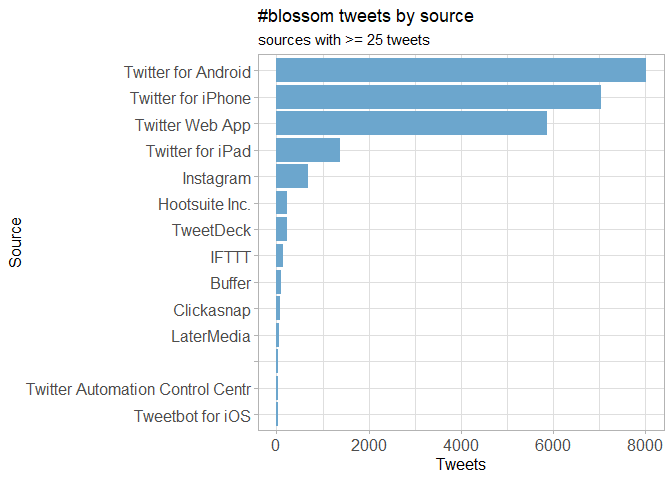
\includegraphics{twitter-blossom-watch-2021_files/figure-latex/tweets-top-sources-1.pdf}

\hypertarget{network-replies}{%
\subsection{Network Replies}\label{network-replies}}

The ``replies network'', composed from users who reply directly to one
another where the hashtag or keyword of blossom was part of the message
text. Complied on Friday 19th March.

\includegraphics{images/repliesnetwork.png}

\hypertarget{network-mentions}{%
\subsection{Network Mentions}\label{network-mentions}}

The ``mentions network'' is where users mention other users in their
tweets and those tweets contain a keyword such as blossom. The large
network (mid-right) is the National Trust twitter account. The smaller
networks are key influencers that have shared blossom tweets with their
network which have subsequently shared it to their followers too.

\includegraphics{images/mentionsnetwork.png}

\hypertarget{retweets}{%
\section{Retweets}\label{retweets}}

\hypertarget{top-retweets}{%
\subsection{Top retweets}\label{top-retweets}}

Top re-tweeters and total re-tweet counts.

\begin{longtable}[]{@{}llr@{}}
\toprule
\begin{minipage}[b]{0.22\columnwidth}\raggedright
screen\_name\strut
\end{minipage} & \begin{minipage}[b]{0.49\columnwidth}\raggedright
text\strut
\end{minipage} & \begin{minipage}[b]{0.20\columnwidth}\raggedleft
retweet\_count\strut
\end{minipage}\tabularnewline
\midrule
\endhead
\begin{minipage}[t]{0.22\columnwidth}\raggedright
nationaltrust\strut
\end{minipage} & \begin{minipage}[t]{0.49\columnwidth}\raggedright
Pause to soak up the sweet scents and soft songs emanating from blossom
branches. These colourful trees are a feast for the senses.
\#BlossomWatch \url{https://t.co/GsXfF5KPAE}\strut
\end{minipage} & \begin{minipage}[t]{0.20\columnwidth}\raggedleft
243\strut
\end{minipage}\tabularnewline
\begin{minipage}[t]{0.22\columnwidth}\raggedright
DrDarrenRFlower\strut
\end{minipage} & \begin{minipage}[t]{0.49\columnwidth}\raggedright
Central Park New York \#spring \#spring2021 \#blossom \#cherry
\url{https://t.co/Oimq2hRU1k}\strut
\end{minipage} & \begin{minipage}[t]{0.20\columnwidth}\raggedleft
152\strut
\end{minipage}\tabularnewline
\begin{minipage}[t]{0.22\columnwidth}\raggedright
nationaltrust\strut
\end{minipage} & \begin{minipage}[t]{0.49\columnwidth}\raggedright
Happily dancing in the breeze, a golden daffodil is full of cheer.
\#EveryoneNeedsNature \url{https://t.co/hSOWdCCnPL}\strut
\end{minipage} & \begin{minipage}[t]{0.20\columnwidth}\raggedleft
122\strut
\end{minipage}\tabularnewline
\begin{minipage}[t]{0.22\columnwidth}\raggedright
nationaltrust\strut
\end{minipage} & \begin{minipage}[t]{0.49\columnwidth}\raggedright
Everywhere these delicate flowers emerge, they bring delight with them.
Thanks to everyone who's helped spread the joys of blossom so far - keep
the photos coming with \#BlossomWatch. Photos: Joanna A, Catherine A,
Shonali B, Cara W. \url{https://t.co/6znNDEdvKC}\strut
\end{minipage} & \begin{minipage}[t]{0.20\columnwidth}\raggedleft
122\strut
\end{minipage}\tabularnewline
\begin{minipage}[t]{0.22\columnwidth}\raggedright
nationaltrust\strut
\end{minipage} & \begin{minipage}[t]{0.49\columnwidth}\raggedright
\textless U+0001F338\textgreater\#BlossomWatch\textless U+0001F338\textgreater{}
Lockdowns have changed the nation's relationship with nature for the
better. We are feeling more connected thanks to our daily strolls and
taking more notice of the changing seasons.
\url{https://t.co/JtIkqgUorV}\strut
\end{minipage} & \begin{minipage}[t]{0.20\columnwidth}\raggedleft
100\strut
\end{minipage}\tabularnewline
\begin{minipage}[t]{0.22\columnwidth}\raggedright
MikeDoylePhotos\strut
\end{minipage} & \begin{minipage}[t]{0.49\columnwidth}\raggedright
Autumnal view at Sheffield Park, East Sussex. \#Sussex \#England
\#NationalTrust \#landscape \#landscapephotography \#travel
\#travelphotography \#photo \#photography \#photooftheday
\#NaturePhotography \url{https://t.co/FqII3JWs8w}\strut
\end{minipage} & \begin{minipage}[t]{0.20\columnwidth}\raggedleft
97\strut
\end{minipage}\tabularnewline
\begin{minipage}[t]{0.22\columnwidth}\raggedright
nationaltrust\strut
\end{minipage} & \begin{minipage}[t]{0.49\columnwidth}\raggedright
When you see the blossom dancing in the breeze, pause to notice the
bewitching perfume drifting along with it. \#BlossomWatch
\url{https://t.co/Kh68Hh3iMx}\strut
\end{minipage} & \begin{minipage}[t]{0.20\columnwidth}\raggedleft
78\strut
\end{minipage}\tabularnewline
\begin{minipage}[t]{0.22\columnwidth}\raggedright
nationaltrust\strut
\end{minipage} & \begin{minipage}[t]{0.49\columnwidth}\raggedright
One of life's simple pleasures that can be enjoyed from anywhere.
Engross yourself in the calming colours of a sunrise.
\#EveryoneNeedsNature \url{https://t.co/l5xkDICUPn}\strut
\end{minipage} & \begin{minipage}[t]{0.20\columnwidth}\raggedleft
72\strut
\end{minipage}\tabularnewline
\begin{minipage}[t]{0.22\columnwidth}\raggedright
ampomata\strut
\end{minipage} & \begin{minipage}[t]{0.49\columnwidth}\raggedright
This is my new painting ``Bed Of Roses''. You can check it out here:
\url{https://t.co/GoYnqeM1YY} \#art \#arte \#oleo \#kunst \#oilpainting
\#contemporaryart \#ArtistOnTwitter \#blossom \#flower \#floral \#spring
\#pink \#red \#roses \#field \#artprints \#flowers \#garden
\url{https://t.co/7y9skbUaMs}\strut
\end{minipage} & \begin{minipage}[t]{0.20\columnwidth}\raggedleft
69\strut
\end{minipage}\tabularnewline
\begin{minipage}[t]{0.22\columnwidth}\raggedright
MikeDoylePhotos\strut
\end{minipage} & \begin{minipage}[t]{0.49\columnwidth}\raggedright
Early autumn at Sheffield Park, East Sussex. \#Sussex \#England
\#NationalTrust \#landscape \#landscapephotography \#travel
\#travelphotography \#photo \#photography \#photooftheday
\#NaturePhotography \url{https://t.co/fqSC6f0xMQ}\strut
\end{minipage} & \begin{minipage}[t]{0.20\columnwidth}\raggedleft
64\strut
\end{minipage}\tabularnewline
\bottomrule
\end{longtable}

\hypertarget{favourites}{%
\section{Favourites}\label{favourites}}

\hypertarget{favourite-proportion}{%
\subsection{Favourite proportion}\label{favourite-proportion}}

How many times a tweet was saved a favourite that contained the blossom
keywords.
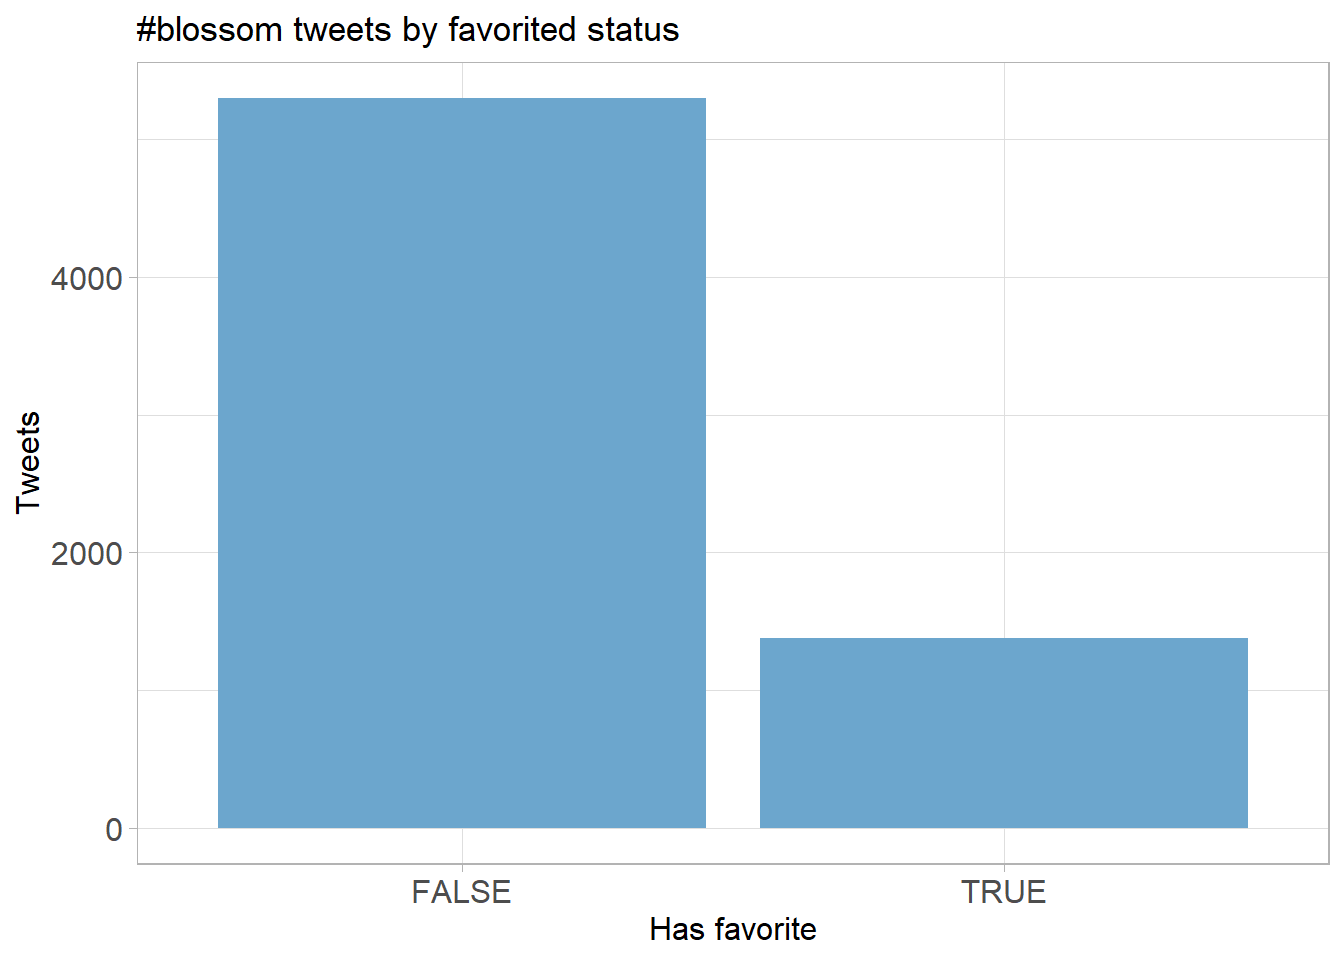
\includegraphics{twitter-blossom-watch-2021_files/figure-latex/has-favorite-1.pdf}

\hypertarget{top-favourites}{%
\subsection{Top favourites}\label{top-favourites}}

\begin{longtable}[]{@{}llr@{}}
\toprule
\begin{minipage}[b]{0.22\columnwidth}\raggedright
screen\_name\strut
\end{minipage} & \begin{minipage}[b]{0.49\columnwidth}\raggedright
text\strut
\end{minipage} & \begin{minipage}[b]{0.21\columnwidth}\raggedleft
favorite\_count\strut
\end{minipage}\tabularnewline
\midrule
\endhead
\begin{minipage}[t]{0.22\columnwidth}\raggedright
nationaltrust\strut
\end{minipage} & \begin{minipage}[t]{0.49\columnwidth}\raggedright
Pause to soak up the sweet scents and soft songs emanating from blossom
branches. These colourful trees are a feast for the senses.
\#BlossomWatch \url{https://t.co/GsXfF5KPAE}\strut
\end{minipage} & \begin{minipage}[t]{0.21\columnwidth}\raggedleft
1127\strut
\end{minipage}\tabularnewline
\begin{minipage}[t]{0.22\columnwidth}\raggedright
DrDarrenRFlower\strut
\end{minipage} & \begin{minipage}[t]{0.49\columnwidth}\raggedright
Central Park New York \#spring \#spring2021 \#blossom \#cherry
\url{https://t.co/Oimq2hRU1k}\strut
\end{minipage} & \begin{minipage}[t]{0.21\columnwidth}\raggedleft
835\strut
\end{minipage}\tabularnewline
\begin{minipage}[t]{0.22\columnwidth}\raggedright
nationaltrust\strut
\end{minipage} & \begin{minipage}[t]{0.49\columnwidth}\raggedright
Everywhere these delicate flowers emerge, they bring delight with them.
Thanks to everyone who's helped spread the joys of blossom so far - keep
the photos coming with \#BlossomWatch. Photos: Joanna A, Catherine A,
Shonali B, Cara W. \url{https://t.co/6znNDEdvKC}\strut
\end{minipage} & \begin{minipage}[t]{0.21\columnwidth}\raggedleft
697\strut
\end{minipage}\tabularnewline
\begin{minipage}[t]{0.22\columnwidth}\raggedright
nationaltrust\strut
\end{minipage} & \begin{minipage}[t]{0.49\columnwidth}\raggedright
Happily dancing in the breeze, a golden daffodil is full of cheer.
\#EveryoneNeedsNature \url{https://t.co/hSOWdCCnPL}\strut
\end{minipage} & \begin{minipage}[t]{0.21\columnwidth}\raggedleft
691\strut
\end{minipage}\tabularnewline
\begin{minipage}[t]{0.22\columnwidth}\raggedright
MikeDoylePhotos\strut
\end{minipage} & \begin{minipage}[t]{0.49\columnwidth}\raggedright
Autumnal view at Sheffield Park, East Sussex. \#Sussex \#England
\#NationalTrust \#landscape \#landscapephotography \#travel
\#travelphotography \#photo \#photography \#photooftheday
\#NaturePhotography \url{https://t.co/FqII3JWs8w}\strut
\end{minipage} & \begin{minipage}[t]{0.21\columnwidth}\raggedleft
631\strut
\end{minipage}\tabularnewline
\begin{minipage}[t]{0.22\columnwidth}\raggedright
nationaltrust\strut
\end{minipage} & \begin{minipage}[t]{0.49\columnwidth}\raggedright
\textless U+0001F338\textgreater\#BlossomWatch\textless U+0001F338\textgreater{}
Lockdowns have changed the nation's relationship with nature for the
better. We are feeling more connected thanks to our daily strolls and
taking more notice of the changing seasons.
\url{https://t.co/JtIkqgUorV}\strut
\end{minipage} & \begin{minipage}[t]{0.21\columnwidth}\raggedleft
597\strut
\end{minipage}\tabularnewline
\begin{minipage}[t]{0.22\columnwidth}\raggedright
MikeDoylePhotos\strut
\end{minipage} & \begin{minipage}[t]{0.49\columnwidth}\raggedright
Early autumn at Sheffield Park, East Sussex. \#Sussex \#England
\#NationalTrust \#landscape \#landscapephotography \#travel
\#travelphotography \#photo \#photography \#photooftheday
\#NaturePhotography \url{https://t.co/fqSC6f0xMQ}\strut
\end{minipage} & \begin{minipage}[t]{0.21\columnwidth}\raggedleft
543\strut
\end{minipage}\tabularnewline
\begin{minipage}[t]{0.22\columnwidth}\raggedright
nationaltrust\strut
\end{minipage} & \begin{minipage}[t]{0.49\columnwidth}\raggedright
Who else is buzzing with excitement at the blossom appearing? We love
hearing the calming hum of bees enjoying the flowers. \#BlossomWatch
Photo: Rosie S, @ClivedenNT \url{https://t.co/JGcihvsoCV}\strut
\end{minipage} & \begin{minipage}[t]{0.21\columnwidth}\raggedleft
536\strut
\end{minipage}\tabularnewline
\begin{minipage}[t]{0.22\columnwidth}\raggedright
JuliaBradbury\strut
\end{minipage} & \begin{minipage}[t]{0.49\columnwidth}\raggedright
Spending time to dwell on nature can improve your wellbeing- research
shows that just 20 mins can improve your mood.Only 6\% take the time to
celebrate things like the first seasonal first day of spring.
@nationaltrust is helping to plant more blossom trees \#BlossomWatch
\#hanami \url{https://t.co/UkuU9I6x91}\strut
\end{minipage} & \begin{minipage}[t]{0.21\columnwidth}\raggedleft
523\strut
\end{minipage}\tabularnewline
\begin{minipage}[t]{0.22\columnwidth}\raggedright
nationaltrust\strut
\end{minipage} & \begin{minipage}[t]{0.49\columnwidth}\raggedright
When you see the blossom dancing in the breeze, pause to notice the
bewitching perfume drifting along with it. \#BlossomWatch
\url{https://t.co/Kh68Hh3iMx}\strut
\end{minipage} & \begin{minipage}[t]{0.21\columnwidth}\raggedleft
455\strut
\end{minipage}\tabularnewline
\bottomrule
\end{longtable}

\hypertarget{quotes}{%
\section{Quotes}\label{quotes}}

\hypertarget{top-quotes}{%
\subsection{Top quotes}\label{top-quotes}}

Joining, by = ``quoted\_status\_id''

\begin{longtable}[]{@{}llr@{}}
\toprule
\begin{minipage}[b]{0.23\columnwidth}\raggedright
screen\_name\strut
\end{minipage} & \begin{minipage}[b]{0.42\columnwidth}\raggedright
text\strut
\end{minipage} & \begin{minipage}[b]{0.18\columnwidth}\raggedleft
quote\_count\strut
\end{minipage}\tabularnewline
\midrule
\endhead
\begin{minipage}[t]{0.23\columnwidth}\raggedright
Ms\_SJP\strut
\end{minipage} & \begin{minipage}[t]{0.42\columnwidth}\raggedright
Well the National Trust's \#blossomwatch hashtag is my new favourite
thing, I have to say! \textless U+0001F338\textgreater{}
\url{https://t.co/i4cj9FF1VX}\strut
\end{minipage} & \begin{minipage}[t]{0.18\columnwidth}\raggedleft
4\strut
\end{minipage}\tabularnewline
\begin{minipage}[t]{0.23\columnwidth}\raggedright
LBGAmbEast\strut
\end{minipage} & \begin{minipage}[t]{0.42\columnwidth}\raggedright
Some wonderful images on @nationaltrust's \#BlossomWatch thread
\url{https://t.co/1XSkaKnQZc}\strut
\end{minipage} & \begin{minipage}[t]{0.18\columnwidth}\raggedleft
4\strut
\end{minipage}\tabularnewline
\begin{minipage}[t]{0.23\columnwidth}\raggedright
NaturalEngland\strut
\end{minipage} & \begin{minipage}[t]{0.42\columnwidth}\raggedright
Our research shows that nature is more important than ever to us since
the pandemic started. We're taking more notice of small changes in
nature and signs of spring, like beautiful apple blossom. Share your
pictures of blossom with @NationalTrust using
\textless U+0001F338\textgreater\#BlossomWatch
\textless U+0001F338\textgreater{} \url{https://t.co/KlDTIYa46E}\strut
\end{minipage} & \begin{minipage}[t]{0.18\columnwidth}\raggedleft
4\strut
\end{minipage}\tabularnewline
\begin{minipage}[t]{0.23\columnwidth}\raggedright
radiowinch\strut
\end{minipage} & \begin{minipage}[t]{0.42\columnwidth}\raggedright
Spring is on the way. Celebrate the arrival of blossom near you with
\#BlossomWatch share your photos \url{https://t.co/B0TuHmf6Sk}\strut
\end{minipage} & \begin{minipage}[t]{0.18\columnwidth}\raggedleft
4\strut
\end{minipage}\tabularnewline
\begin{minipage}[t]{0.23\columnwidth}\raggedright
JamesGardening\strut
\end{minipage} & \begin{minipage}[t]{0.42\columnwidth}\raggedright
Share with everyone your blossom pics using the \#BlossomWatch and
national trust. plenty of amazing pictures to view.
\url{https://t.co/57ZDpy4865}\strut
\end{minipage} & \begin{minipage}[t]{0.18\columnwidth}\raggedleft
3\strut
\end{minipage}\tabularnewline
\begin{minipage}[t]{0.23\columnwidth}\raggedright
SpiralStripeArt\strut
\end{minipage} & \begin{minipage}[t]{0.42\columnwidth}\raggedright
Loving the @nationaltrust latest campaign \#BlossomWatch which I know my
\#SMM friends will appreciate as a brilliant example of user-generated
content! \textless U+0001F338\textgreater{} The campaign has even been
advertised on \textless U+0001F4FA\textgreater{} @1OFFGINGER
@sociallymaz @TechPixies @hellosocialLdn @muchmoresocial
\url{https://t.co/EGyVKh0Vht}\strut
\end{minipage} & \begin{minipage}[t]{0.18\columnwidth}\raggedleft
3\strut
\end{minipage}\tabularnewline
\begin{minipage}[t]{0.23\columnwidth}\raggedright
heritage\_lizzie\strut
\end{minipage} & \begin{minipage}[t]{0.42\columnwidth}\raggedright
Yes! Here’s magnolia on the school run today \#blossomwatch My
favourite time of year. @nationaltrust \url{https://t.co/7nq3iQrw5J}
\url{https://t.co/Mg7BMMOZ4V}\strut
\end{minipage} & \begin{minipage}[t]{0.18\columnwidth}\raggedleft
3\strut
\end{minipage}\tabularnewline
\begin{minipage}[t]{0.23\columnwidth}\raggedright
wearealtervego\strut
\end{minipage} & \begin{minipage}[t]{0.42\columnwidth}\raggedright
Taking in the \#nature around us\ldots\#andbreathe \#blossomwatch
\#savethebees \#savetheworld \url{https://t.co/9OKBi1ot9E}\strut
\end{minipage} & \begin{minipage}[t]{0.18\columnwidth}\raggedleft
2\strut
\end{minipage}\tabularnewline
\begin{minipage}[t]{0.23\columnwidth}\raggedright
GillianFoxcroft\strut
\end{minipage} & \begin{minipage}[t]{0.42\columnwidth}\raggedright
Wonderful initiative by @nationaltrust Lucky enough to live near
@KedlestonNT where this blackthorn was heralding spring, but blossom is
accessible in our towns and cities too \#BlossomWatch
\url{https://t.co/l3nMn9dvGe} \url{https://t.co/Nri4nxd3vL}\strut
\end{minipage} & \begin{minipage}[t]{0.18\columnwidth}\raggedleft
2\strut
\end{minipage}\tabularnewline
\begin{minipage}[t]{0.23\columnwidth}\raggedright
weather2travel\strut
\end{minipage} & \begin{minipage}[t]{0.42\columnwidth}\raggedright
Will you be joining @nationaltrust \#BlossomWatch?
\textless U+0001F338\textgreater\textless U+0001F440\textgreater{}
\#thursdaymorning \#ThoughtForTheDay \#spring \#bliss
\url{https://t.co/aiQYIY1n5N}\strut
\end{minipage} & \begin{minipage}[t]{0.18\columnwidth}\raggedleft
2\strut
\end{minipage}\tabularnewline
\bottomrule
\end{longtable}

\hypertarget{media}{%
\section{Media}\label{media}}

\hypertarget{media-count}{%
\subsection{Media count}\label{media-count}}

Shows tweets where a piece of media was shared such as images or videos.
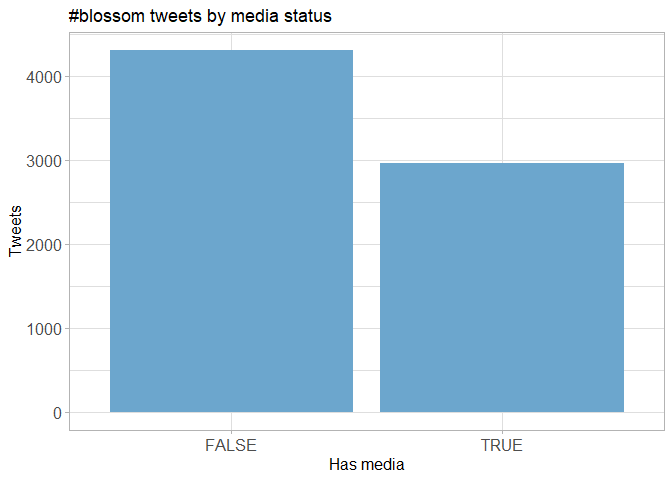
\includegraphics{twitter-blossom-watch-2021_files/figure-latex/has-media-1.pdf}

\hypertarget{top-media}{%
\subsection{Top media}\label{top-media}}

\begin{longtable}[]{@{}llr@{}}
\toprule
\begin{minipage}[b]{0.22\columnwidth}\raggedright
screen\_name\strut
\end{minipage} & \begin{minipage}[b]{0.49\columnwidth}\raggedright
text\strut
\end{minipage} & \begin{minipage}[b]{0.21\columnwidth}\raggedleft
favorite\_count\strut
\end{minipage}\tabularnewline
\midrule
\endhead
\begin{minipage}[t]{0.22\columnwidth}\raggedright
nationaltrust\strut
\end{minipage} & \begin{minipage}[t]{0.49\columnwidth}\raggedright
Pause to soak up the sweet scents and soft songs emanating from blossom
branches. These colourful trees are a feast for the senses.
\#BlossomWatch \url{https://t.co/GsXfF5KPAE}\strut
\end{minipage} & \begin{minipage}[t]{0.21\columnwidth}\raggedleft
1127\strut
\end{minipage}\tabularnewline
\begin{minipage}[t]{0.22\columnwidth}\raggedright
DrDarrenRFlower\strut
\end{minipage} & \begin{minipage}[t]{0.49\columnwidth}\raggedright
Central Park New York \#spring \#spring2021 \#blossom \#cherry
\url{https://t.co/Oimq2hRU1k}\strut
\end{minipage} & \begin{minipage}[t]{0.21\columnwidth}\raggedleft
835\strut
\end{minipage}\tabularnewline
\begin{minipage}[t]{0.22\columnwidth}\raggedright
nationaltrust\strut
\end{minipage} & \begin{minipage}[t]{0.49\columnwidth}\raggedright
Everywhere these delicate flowers emerge, they bring delight with them.
Thanks to everyone who's helped spread the joys of blossom so far - keep
the photos coming with \#BlossomWatch. Photos: Joanna A, Catherine A,
Shonali B, Cara W. \url{https://t.co/6znNDEdvKC}\strut
\end{minipage} & \begin{minipage}[t]{0.21\columnwidth}\raggedleft
697\strut
\end{minipage}\tabularnewline
\begin{minipage}[t]{0.22\columnwidth}\raggedright
nationaltrust\strut
\end{minipage} & \begin{minipage}[t]{0.49\columnwidth}\raggedright
Happily dancing in the breeze, a golden daffodil is full of cheer.
\#EveryoneNeedsNature \url{https://t.co/hSOWdCCnPL}\strut
\end{minipage} & \begin{minipage}[t]{0.21\columnwidth}\raggedleft
691\strut
\end{minipage}\tabularnewline
\begin{minipage}[t]{0.22\columnwidth}\raggedright
MikeDoylePhotos\strut
\end{minipage} & \begin{minipage}[t]{0.49\columnwidth}\raggedright
Autumnal view at Sheffield Park, East Sussex. \#Sussex \#England
\#NationalTrust \#landscape \#landscapephotography \#travel
\#travelphotography \#photo \#photography \#photooftheday
\#NaturePhotography \url{https://t.co/FqII3JWs8w}\strut
\end{minipage} & \begin{minipage}[t]{0.21\columnwidth}\raggedleft
631\strut
\end{minipage}\tabularnewline
\begin{minipage}[t]{0.22\columnwidth}\raggedright
nationaltrust\strut
\end{minipage} & \begin{minipage}[t]{0.49\columnwidth}\raggedright
\textless U+0001F338\textgreater\#BlossomWatch\textless U+0001F338\textgreater{}
Lockdowns have changed the nation's relationship with nature for the
better. We are feeling more connected thanks to our daily strolls and
taking more notice of the changing seasons.
\url{https://t.co/JtIkqgUorV}\strut
\end{minipage} & \begin{minipage}[t]{0.21\columnwidth}\raggedleft
597\strut
\end{minipage}\tabularnewline
\begin{minipage}[t]{0.22\columnwidth}\raggedright
MikeDoylePhotos\strut
\end{minipage} & \begin{minipage}[t]{0.49\columnwidth}\raggedright
Early autumn at Sheffield Park, East Sussex. \#Sussex \#England
\#NationalTrust \#landscape \#landscapephotography \#travel
\#travelphotography \#photo \#photography \#photooftheday
\#NaturePhotography \url{https://t.co/fqSC6f0xMQ}\strut
\end{minipage} & \begin{minipage}[t]{0.21\columnwidth}\raggedleft
543\strut
\end{minipage}\tabularnewline
\begin{minipage}[t]{0.22\columnwidth}\raggedright
nationaltrust\strut
\end{minipage} & \begin{minipage}[t]{0.49\columnwidth}\raggedright
Who else is buzzing with excitement at the blossom appearing? We love
hearing the calming hum of bees enjoying the flowers. \#BlossomWatch
Photo: Rosie S, @ClivedenNT \url{https://t.co/JGcihvsoCV}\strut
\end{minipage} & \begin{minipage}[t]{0.21\columnwidth}\raggedleft
536\strut
\end{minipage}\tabularnewline
\begin{minipage}[t]{0.22\columnwidth}\raggedright
JuliaBradbury\strut
\end{minipage} & \begin{minipage}[t]{0.49\columnwidth}\raggedright
Spending time to dwell on nature can improve your wellbeing- research
shows that just 20 mins can improve your mood.Only 6\% take the time to
celebrate things like the first seasonal first day of spring.
@nationaltrust is helping to plant more blossom trees \#BlossomWatch
\#hanami \url{https://t.co/UkuU9I6x91}\strut
\end{minipage} & \begin{minipage}[t]{0.21\columnwidth}\raggedleft
523\strut
\end{minipage}\tabularnewline
\begin{minipage}[t]{0.22\columnwidth}\raggedright
nationaltrust\strut
\end{minipage} & \begin{minipage}[t]{0.49\columnwidth}\raggedright
When you see the blossom dancing in the breeze, pause to notice the
bewitching perfume drifting along with it. \#BlossomWatch
\url{https://t.co/Kh68Hh3iMx}\strut
\end{minipage} & \begin{minipage}[t]{0.21\columnwidth}\raggedleft
455\strut
\end{minipage}\tabularnewline
\bottomrule
\end{longtable}

\hypertarget{most-liked-media-image}{%
\subsubsection{Most liked media image}\label{most-liked-media-image}}

\includegraphics{list("http://pbs.twimg.com/ext_tw_video_thumb/1373173799307345922/pu/img/Qcm5UVfXdZyyCNjR.jpg")}

\hypertarget{tweet-text}{%
\section{Tweet text}\label{tweet-text}}

The top 150 words used 3 or more times within tweet which contain
keywords around blossom. Words removed: blossom, blossomwatch,
nationaltrust, everyoneneedsnature.

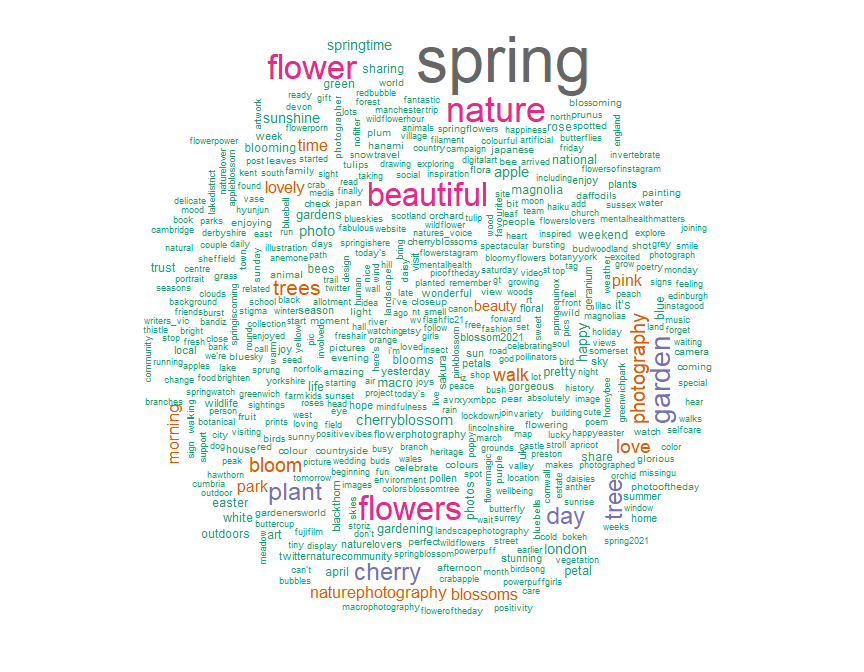
\includegraphics{twitter-blossom-watch-2021_files/figure-latex/count-words-1.pdf}

\hypertarget{tweets-by-tweet-length}{%
\subsection{Tweets by Tweet Length}\label{tweets-by-tweet-length}}

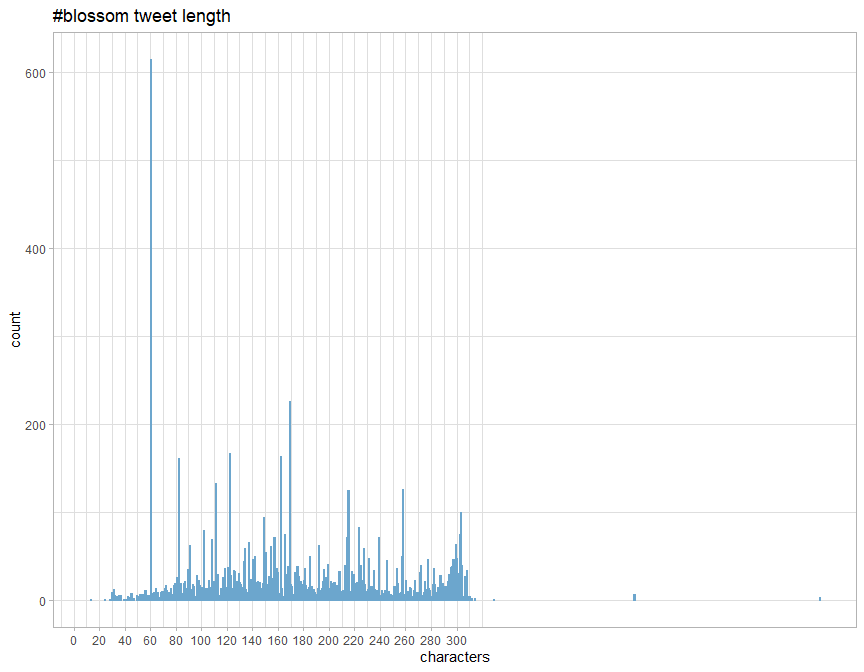
\includegraphics{twitter-blossom-watch-2021_files/figure-latex/count-tweet-length-1.pdf}

\hypertarget{blossom-sentiment-analysis---visualisation}{%
\subsection{Blossom Sentiment Analysis -
Visualisation}\label{blossom-sentiment-analysis---visualisation}}

This process analyses each word within the tweet and then categorises
the tweet into one of 8 main categories and polarity. Each triangle in
the plot is a tweet where one of the blossom keywords was found and the
overall tweet was categorised. Blossom related tweets show strong
`positive' and `joy' correlations based on the language used by
tweeters.
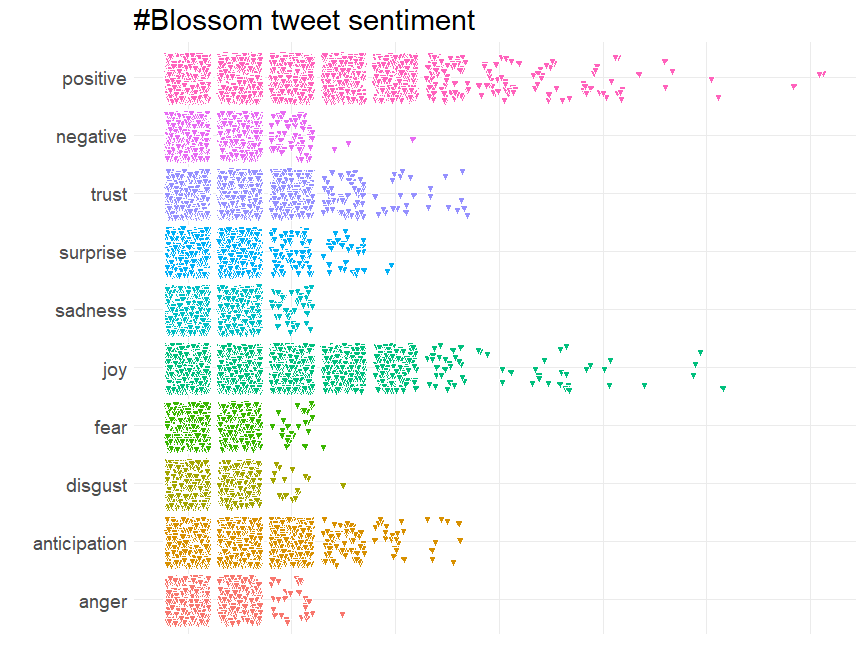
\includegraphics{twitter-blossom-watch-2021_files/figure-latex/sentiment-analysis-1.pdf}

\end{document}
